\documentclass[aps,preprint,tightenlines,floatfix,superscriptaddress,nofootinbib,showpacs]{revtex4-1}
\pdfoutput=1
\usepackage{graphicx}
%\usepackage{dcolumn}
\usepackage{amsfonts}
\usepackage{hhline}
\usepackage{multirow}
\usepackage{array}
\usepackage{dsfont}
%\usepackage{longtable}
%\usepackage{amsmath}
\usepackage{amssymb}
\usepackage{maybemath}
%\usepackage[italic]{hepparticles}
\usepackage{float}
\usepackage[lofdepth,lotdepth]{subfig}
\usepackage[countmax]{subfloat}
\usepackage{cancel}
%\usepackage[nodisplayskipstretch]{setspace}
%\setstretch{1.5}
%\usepackage{caption}
%\usepackage{subcaption}
\setlength{\oddsidemargin}{-1in}
\addtolength{\oddsidemargin}{24mm} \setlength{\textwidth}{170mm}
\setlength{\topmargin}{-0.55in} \setlength{\headheight}{10mm}
\setlength{\headsep}{0mm} \setlength{\textheight}{230mm}
\def\beq{\begin{equation}}
\def\eeq{\end{equation}}
\def\bea{\begin{eqnarray}}
\def\eea{\end{eqnarray}}
\def\nn{\nonumber}
\def\sss{\scriptstyle}
\def\lft{{\scriptstyle L}}
\def\rht{{\scriptstyle R}}
\def\roughly#1{\mathrel{\raise.3ex\hbox
{$#1$\kern-.75em\lower1ex\hbox{$\sim$}}}}
\def\lsim{\roughly<}
\def\gsim{\roughly>}
\def\tbslash{\tbar\hspace{-10pt}\not{}\hspace{4pt}}
\def\pslash{p\hspace{-10pt}\not{}\hspace{2pt}}
\def\kslash{k\hspace{-11pt}\not{}\hspace{2pt}}
\def\qslash{q\hspace{-10pt}\not{}\hspace{2pt}}
\def\rslash{r\hspace{-10pt}\not{}\hspace{2pt}}
\def\Qslash{\not{}\hspace{-4pt}\tilde{Q}}
\def\tslash{t\hspace{-10pt}\not{}\hspace{4pt}}
\def\lpslash{l^+\hspace{-10pt}\not{}\hspace{4pt}}
\def\lmslash{l^-\hspace{-10pt}\not{}\hspace{4pt}}
\def\nslash{n\hspace{-10pt}\not{}\hspace{4pt}}
\def\ntbslash{n_{\tbar}\hspace{-10pt}\not{}\hspace{4pt}}
%%%%%%%%%%%%%%%%%%%%%%%%%%%%%%%%%%%%%%%%%%%%%%%%%%%%%%%%%%%%%%%%%%%%%%%%%%%%%%%
\newcommand{\note}[1]{\marginpar{{\small\begin{center}{\it #1}\end{center}}}}
\newcommand*\xbar[1]{%
  \hbox{%
    \vbox{%
      \hrule height 0.5pt % The actual bar
      \kern0.3ex%         % Distance between bar and symbol
      \hbox{%
        \kern-0.1em%      % Shortening on the left side
        \ensuremath{#1}%
        \kern-0.1em%      % Shortening on the right side
      }%
    }%
  }%
} 
\newcommand{\unit}{1\!\!1}
%%%%%%%%%%%%%%%%%%%%%%%%%%%%%%%%%%%%%%%%%%%%%%%%%%%%%%%%%%%%%%%%%%%%%%%%%%%%%%%
\def\tbar{\bar{t}}
%\def\tbar{{\overline{t}}}
\def\bbar{\bar{b}}
\def\qbar{\bar{q}}
\def\nubar{{\bar{\nu}}_{\ell}}
\def\tbbc{t \to b \bbar c}
\def\tauprocess{\tau\rightarrow K\pi\pi\nu_{\tau}}
\def\ppprocess{pp\to t\,\left(\rightarrow b {\ell}^+ \nu_{\ell}\right) \tbar\,\left(\rightarrow\bbar {\ell}^-\nubar\right)\,H}
\def\bppprocess{{\boldmath $pp\to t \tbar H\to \left(b {\ell}^+ \nu_{\ell}\right)\left(\bbar {\ell}^-\nubar\right)H$}}
\def\ggprocess{gg\to t \tbar H\to\left(b l^+ \nu_l\right)\left(\bbar l^-\nubar\right)H}
\def\qqprocess{q\qbar\to t \tbar H\to\left(b l^+ \nu_l\right)\left(\bbar l^-\nubar\right)H}
\def\kp{\kappa_t}
\def\kpt{\tilde{\kappa}_t}
\def\MG{\mbox{MadGraph 5}}
\def\tm#1{\texttt{TM-{#1}}}
\def\ex#1{\texttt{EX-{#1}}}
\def\Ahat{\hat A_i^{\sigma}}
\def\madg{MadGraph~5}
\def\TPa{\epsilon(t,\tbar,n_t,n_{\tbar})}
\def\TPb{\epsilon(Q,\tbar,n_t,n_{\tbar})}
\def\TPc{\epsilon(Q,t,n_t,n_{\tbar})}
%%%%%%%%%%%%%%%%%%%%%%%%%%%%%%%%%%%%%%%%%%%%%%%%%%%%%%%%%%%%%%%%%%%%%%%%
%%%%%
%for editing purposes
\usepackage[normalem]{ulem}
\usepackage{color}
\definecolor{BrickRed}{cmyk}{0,0.89,0.94,0.28}
\definecolor{DarkGreen}{cmyk}{1,0,1,0.5}
\definecolor{Blue}{cmyk}{1,1,0,0}
\definecolor{BurntOrange}{cmyk}{0,0.51,1,0}

\def\hldl#1{\textcolor{BrickRed}{\textsf{#1}}}
\def\hlps#1{\textcolor{DarkGreen}{\textsf{#1}}}
\def\hlkk#1{\textcolor{Blue}{\textsf{#1}}}
\def\hlas#1{\textcolor{BurntOrange}{\textsf{#1}}}
\def\soutdl{\bgroup\markoverwith{\textcolor{BrickRed}{\rule[0.5ex]{2pt}{0.4pt}}}\ULon}
\def\soutps{\bgroup\markoverwith{\textcolor{DarkGreen}{\rule[0.5ex]{2pt}{0.4pt}}}\ULon}
\def\soutkk{\bgroup\markoverwith{\textcolor{Blue}{\rule[0.5ex]{2pt}{0.4pt}}}\ULon}
\def\soutas{\bgroup\markoverwith{\textcolor{BurntOrange}{\rule[0.5ex]{2pt}{0.4pt}}}\ULon}

\def\mhldl#1{\textcolor{BrickRed}{\ensuremath{#1}}}
\def\mhlps#1{\textcolor{DarkGreen}{\ensuremath{#1}}}
\def\mhlkk#1{\textcolor{Blue}{\ensuremath{#1}}}
\def\mhlas#1{\textcolor{BurntOrange}{\ensuremath{#1}}}
\def\msoutdl#1{\text{\soutps{\ensuremath{#1}}}}
\def\msoutps#1{\text{\soutps{\ensuremath{#1}}}}
\def\msoutkk#1{\text{\soutps{\ensuremath{#1}}}}
\def\msoutas#1{\text{\soutps{\ensuremath{#1}}}}
%%%%%%%%%%%%%%%%%%%%%%%%%%%%%%%%%%%%%%%%%%%%%%%%%%%%%%%%%%%%%%%%%%%%%%%%
\begin{document}
\vspace*{2cm}

\title{{\boldmath Notes on LQ project I}}

%\def\tayloru{\affiliation{\it Physics and Engineering Department,
%    Taylor University, \\ 236 West Reade Ave., Upland, IN 46989, USA \vspace*{1mm}}}

%\def\tayloru{\affiliation{\it Physics and Engineering Department,
%    Taylor University, \\ 236 West Reade Ave., Upland, IN 46989, USA \vspace*{8mm}}}

\def\laplata{\affiliation{\it IFLP, CONICET -- Dpto. de F\'{\i}sica,
    Universidad Nacional de La Plata, C.C. 67, 1900 La Plata,
    Argentina \vspace*{8mm}}}

\author{Nicolas Mileo}
\email{mileo@fisica.unlp.edu.ar}
\laplata

%\author{Ken Kiers}
%\email{knkiers@taylor.edu}
%\tayloru

\author{Alejandro Szynkman}
\email{szynkman@fisica.unlp.edu.ar}
\laplata

\date{\vspace*{2mm}\today \\\bigskip\bigskip}
\maketitle
%%%%%%%%%%%%%%%%%%%%%%%%%%%%%%%%%%%%%%%%%%%%%%%%%
\section{Standard Model Cross Section}
Within the Standard Model (SM) there are two types of interaction between the incoming neutrino and the nucleons in the detector that are the most relevant in order to understand the signal events collected in IceCube, namely the charged current process (C.C. process) in which the interaction between the neutrino and the nucleon proceeds via the exchange of a W boson and the neutral current process (N.C. process) in which a Z boson is exchanged \cite{Gandhi}.\par Let us first compute the cross section for the C.C. process $\nu_{\ell} N \rightarrow \ell^- + \mbox{anything}$. The relevant dominant diagrams at parton level are shown in Fig.~\ref{fig1} where $\ell =e,\mu,\tau$, the index $i$ denotes the quark flavor and $\tilde{Q}=p-q$.
\begin{center}
\begin{figure}[H]
\centering
%\hspace*{-0.4cm}
\subfloat{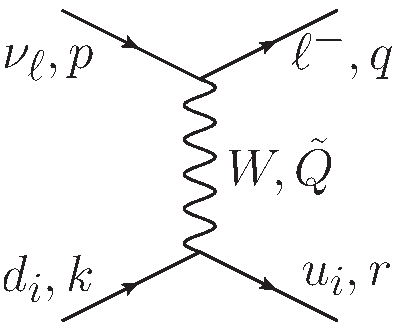
\includegraphics[scale=0.55]{CCprocess_1.pdf}}
\hspace*{0.2\textwidth}
%\label{fig1a}}
\subfloat{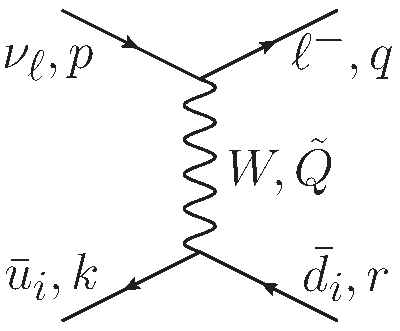
\includegraphics[scale=0.55]{CCprocess_2.pdf}}
%\label{fig1b}}
\caption{Dominant charged current process diagrams. The left diagram shows the scattering of a neutrino by a down-type quark whereas the right diagram depicts the scattering by an up-type antiquark.}
\label{fig1}
\end{figure}
\end{center}
\par
In the case of the first diagram the amplitude is given by
\beq
\label{eq1}
\mathcal{M}(\nu_{\ell}d_i \rightarrow \ell^- u_i)=\left(\!-\frac{ig}{\sqrt{2}}\right)^2 [\bar{u}(q)\gamma_{\mu}\frac{(1-\gamma_5)}{2}u(p)]\,\frac{-i}{\tilde{Q}^2-M^2_W}\left(g^{\mu\nu}-\frac{\tilde{Q}^{\mu}\tilde{Q}^{\nu}}{M^2_W}\right)\,[\bar{u}(r)\gamma_{\nu}\frac{(1-\gamma_5)}{2}u(k)].
\eeq
The contribution proportional to $\tilde{Q}^{\mu}\tilde{Q}^{\nu}/M^2_W$ can be written as 
\beq
\label{eq2}
-\frac{ig^2}{8M^2_W}\frac{1}{\tilde{Q}^2-M^ 2_W}[\bar{u}(q)\Qslash (1-\gamma_5)u(p)]\,[\bar{u}(r)\Qslash (1-\gamma_5)u(k)],
\eeq
and by using $\Qslash = \pslash -\qslash$ along with the Dirac equation for the spinors $\bar{u}(q)$ and $u(p)$, it can be shown that the first term in square brackets is given by
\beq
\label{eq3}
\bar{u}(q)\Qslash (1-\gamma_5)u(p)=-m_{\ell}\bar{u}(q)(1-\gamma_5)u(p).
\eeq
Similarly, the second term in square brackets is proportional to the mass of the quark $u_i$, so that the contribution in Eq.~(\ref{eq2}) is of order $m_l m_{u}/M^2_W$ and then we will neglect it here. Therefore we have
\beq
\label{eq4}
\frac{1}{2}\!\!\!\sum_{\substack{\,\,\,d_i,\, u_i,\, \ell^{-} \\ \tiny{\mathrm{spins}}}}\!\!|\mathcal{M}(\nu_{\ell}d_i \rightarrow \ell^- u_i)|^2=\frac{g^4}{64(\tilde{Q}^2-M^2_W)^2}A^{\mu\nu}B_{\mu \nu},
\eeq
where
\beq
\label{eq5}
A^{\mu\nu}\equiv \sum_{\substack{\ell^-\tiny{\mathrm{spin}}}} [\bar{u}(q)\gamma^{\mu}(1-\gamma_5)u(p)][\bar{u}(p)\gamma^{\nu}(1-\gamma_5)u(q)],
\eeq
\beq
\label{eq6}
B_{\mu\nu}\equiv \frac{1}{2}\sum_{\substack{d_i u_i \\ \tiny{\mathrm{spins}}}} [\bar{u}(r)\gamma_{\mu}(1-\gamma_5)u(k)][\bar{u}(k)\gamma_{\nu}(1-\gamma_5)u(r)],
\eeq
and we have omited the spin indices in the spinors for simplicity. By computing the sums in Eqs.~(\ref{eq5}) and (\ref{eq6}) we obtain
\beq
\label{eq7}
A^{\mu\nu}= 8 \{q^{\mu}p^{\nu} + q^{\nu}p^{\mu} - (q\cdot p)g^{\mu\nu} -i\epsilon^{\mu\nu\alpha\beta} q_{\alpha} p_{\beta} \}
\eeq
\beq
\label{eq8}
B_{\mu\nu}= 4 \{ r_{\mu} k_{\nu}+ r_{\nu} k_{\mu} - (r\cdot k)g_{\mu\nu} - i\epsilon_{\mu\nu\rho\sigma}r^{\rho}k^{\sigma}\}.
\eeq
From the replacement of Eqs.~(\ref{eq7}) and (\ref{eq8}) in Eq.~(\ref{eq4}) we have
\beq
\label{eq9}
|\mathcal{M}|^2_{\mathrm{unpol.}}=\frac{2g^4}{(\tilde{Q}^2-M^2_W)^2}(r\cdot q)(p \cdot k).
\eeq
Since the vector $\tilde{Q}$ is space like, we will use instead the quantity $Q^2 \equiv -\tilde{Q}^2$. On the other hand, by assuming the involved particles as massless the dot products appearing in Eq.~(\ref{eq9}) can be expressed in terms of Mandelstam variables in the following manner
\beq
\label{eq10}
(p\cdot k)=\frac{(p + k)^2}{2}= \frac{\hat{s}}{2}
\eeq
\beq
\label{eq11}
(r\cdot q)=\frac{(r + q)^2}{2}= \frac{\hat{s}}{2}.
\eeq
Hence, the unpolarized squared amplitude can be written as
\beq
\label{eq12}
|\mathcal{M}(\nu_{\ell}d_i \rightarrow \ell^- u_i)|^2_{\mathrm{unpol.}}=\frac{g^4 \hat{s}^2}{2(Q^2+M^2_W)^2}.
\eeq
Let us now compute the Lorentz invariant phase space element. If we consider the center of mass system for simplicity, we have
\beq
\label{eq13}
dLIPS =\frac{1}{2}\frac{1}{4E^2}\frac{1}{2E_{\ell}}\frac{1}{2E_{u}}\frac{d^3q}{(2\pi)^3}\frac{d^3r}{(2\pi)^3} (2\pi)^4 \delta^{(4)}(r+q-p-k),
\eeq
where $E$ denotes the energy of the neutrino and the down type quark in the $\mathrm{CM}$, and $E_{\ell}$ and $E_{u}$ are the energies of the lepton and the up type quark in the same reference frame. By choosing spherical coordinates for the momentum $q$ we have
\beq
\label{eq14}
dLIPS = \frac{1}{8E^2}\frac{1}{2E_{\ell}}\frac{1}{2E_{u}}\frac{1}{(2\pi)^2} |\vec{q}|^2 \sin\theta_{\mathrm{CM}} d\theta_{\mathrm{CM}} d\phi\, d|\vec{q}| \,d^3r \,\delta^{(4)}(r+q-p-k).
\eeq
By integrating in $d^3 r$ and $d\phi$ we obtain
\beq
\nonumber
dLIPS =  \frac{1}{8E^2}\frac{1}{4\tilde{E}^2}\frac{1}{2\pi} d\cos\theta_{\mathrm{CM}} |\vec{q}|^2 \frac{d|\vec{q}|^2}{2}\,\delta (2\tilde{E}-2E) 
\eeq
\beq
\label{eq15}
\,=\frac{1}{2\hat{s}}\frac{1}{16\pi}d\cos\theta_{\mathrm{CM}},\hspace{3cm}
\eeq
where in the last equality we have used that in the $\mathrm{CM}$, $\hat{s}=(2E)^2=4E^2$. Moreover, in the $\mathrm{CM}$ the variable $\hat{t}$ is given by
\beq
\label{eq16}
\hat{t}=(q-p)^2 = (0,E\sin\theta_{\mathrm{CM}},0,E\cos\theta_{\mathrm{CM}}-E)^2=-2E^2(1-\cos\theta_{\mathrm{CM}})=-\hat{s}\frac{(1-\cos\theta_{\mathrm{CM}})}{2},
\eeq
and then $d\hat{t}=(\hat{s}/2)\,d\cos\theta_{\mathrm{CM}}$. Hence, Eq.~(\ref{eq15}) can be written as follows
\beq
\label{eq17}
dLIPS = \frac{d\hat{t}}{16\pi\hat{s}^2}.
\eeq
\par By combining Eqs.~(\ref{eq12}) and (\ref{eq17}) we finally obtain the unpolarized differential cross section for the process $\nu_{\ell}d_i \rightarrow \ell^- u_i$,
\beq
\label{eq18}
\frac{d\sigma}{d\hat{t}}(\nu_{\ell}d_i \rightarrow \ell^- u_i)=\frac{M^4_W}{(Q^2+M^2_W)^2}\frac{G^2_F}{\pi},
\eeq 
where the Fermi constant $G_F$ is defined trough the relation
\beq
\label{eq19}
\frac{G_F}{\sqrt{2}}=\frac{g^2}{8M^2_W}.
\eeq
\par
Let us turn now to the computation of the right diagram of Fig.\ref{fig1}. By neglecting again the contribution proportional to $\tilde{Q}^{\mu}\tilde{Q}^{\nu}/M^2_W$ we have in this case
\beq
\label{eq20}
\frac{1}{2}\!\!\!\sum_{\substack{\,\,\,\bar{u}_i,\, \bar{d}_i,\, \ell^{-} \\ \tiny{\mathrm{spins}}}}\!\!|\mathcal{M}(\nu_{\ell}\bar{u}_i \rightarrow \ell^- \bar{d}_i)|^2=\frac{g^4}{64(\tilde{Q}^2-M^2_W)^2}A^{\mu\nu}\tilde{B}_{\mu \nu},
\eeq
where the tensor $A$ is the same already given in Eq.~(\ref{eq7}) and $\tilde{B}$ is given by
\beq
\label{eq21}
\tilde{B}_{\mu\nu}\equiv \frac{1}{2}\sum_{\substack{\bar{u}_i,\, \bar{d}_i \\ \tiny{\mathrm{spins}}}} [\bar{v}(k)\gamma_{\mu}(1-\gamma_5)v(r)][\bar{v}(r)\gamma_{\nu}(1-\gamma_5)v(k)].
\eeq
The computation of the sum in Eq.~(\ref{eq21}) gives the tensor in Eq.~(\ref{eq8}) but with the momenta $k$ and $r$ interchanged,
\beq
\label{eq22}
\tilde{B}_{\mu\nu}= 4\{k_{\mu}r_{\nu} + k_{\nu}r_{\mu} - (r\cdot k)g_{\mu\nu} - i\epsilon_{\mu\nu\rho\sigma}k^{\rho}r^{\sigma} \}.
\eeq
By inserting Eqs.~(\ref{eq7}) and (\ref{eq21}) in Eq.~(\ref{eq20}) we obtain
\beq
\label{eq23}
|\mathcal{M}|^2_{\mathrm{unpol.}}=\frac{2g^4}{(\tilde{Q}^2-M^2_W)^2}(k\cdot q)(p \cdot r).
\eeq
Again, if we assume that the particles are massless we can write the dot products in Eq.~(\ref{eq23}) in terms of Mandelstam's variables,
\beq
\label{eq24}
(k\cdot q)=-\frac{(k - q)^2}{2}= -\frac{\hat{u}}{2}
\eeq
\beq
\label{eq25}
(p\cdot r)=-\frac{(p - r)^2}{2}= -\frac{\hat{u}}{2}.
\eeq
These relations lead to the following expression for the unpolarized squared amplitude
\beq
\label{eq26}
|\mathcal{M}(\nu_{\ell}\bar{u}_i \rightarrow \ell^- \bar{d}_i)|^2_{\mathrm{unpol.}}=\frac{g^4 \hat{u}^2}{2(Q^2+M^2_W)^2},
\eeq
which combined with Eq.~(\ref{eq17}) gives the corresponding differential cross section,
\beq
\label{eq27}
\frac{d\sigma}{d\hat{t}}(\nu_{\ell}\bar{u}_i \rightarrow \ell^- \bar{d}_i)=\frac{M^4_W}{(Q^2+M^2_W)^2}\frac{G^2_F}{\pi}\left(\frac{\hat{u}}{\hat{s}}\right)^2.
\eeq
\par
Now, it is convenient to express this result in terms of dimensionless combinations of kinematic variables defined in the context of the interaction with a nucleon. If we define the momentum of the nucleon to be $P$, the momentum of a contituent parton can be written as $k=\xi P$ where $\xi$ is the corresponding longitudinal fraction. Similarly, the quantity $\hat{s}$ is given by
\beq
\label{eq28}
\hat{s}=(p+k)^2=2p\cdot k = 2\xi P\cdot p = \xi s
\eeq
with $s$ the squared of the center of mass energy of the system $\nu N$. By assuming the involved partons to be massless, the longitudinal fraction can be obtained in terms of the momenta of the neutrino and the lepton since
\beq
\label{eq29}
0\approx (k+\tilde{Q})^2 = 2k\cdot \tilde{Q} + \tilde{Q}^2 = 2\xi P\cdot \tilde{Q} - Q^2,  
\eeq 
from which
\beq
\label{eq30}
\xi= x, \mbox{ with } x\equiv\frac{Q^2}{2P\cdot \tilde{Q}}\,.
\eeq
Finally, we define the variable $y$ which in the rest frame of the nucleon is the fraction of the neutrino's energy that is transferred to the hadronic system,
\beq
\label{eq31}
y\equiv \frac{2P\cdot\tilde{Q}}{2P\cdot p}=\frac{2k\cdot(p-q)}{2k\cdot p}=\frac{\hat{s}+\hat{u}}{\hat{s}}=1-\frac{\hat{u}}{\hat{s}}.
\eeq
From Eq.~(\ref{eq31}) we obtain the following relation between the Mandelstam variables $\hat{u}$ and $\hat{s}$ of the partons and the dimensionless quantity $y$,
\beq
\label{eq32}
\frac{\hat{u}^2}{\hat{s}^2}=(1-y)^2.
\eeq 
Further, we note that $\hat{t}=-Q^2$. By using the relation in Eq.~(\ref{eq32}) we can write Eq.~(\ref{eq27}) as follows
\beq
\label{eq33}
\frac{d\sigma}{d\hat{t}}(\nu_{\ell}\bar{u}_i \rightarrow \ell^- \bar{d}_i)=\frac{M^4_W}{(Q^2+M^2_W)^2}\frac{G^2_F}{\pi}(1-y)^2.
\eeq
\par
In order to obtain the differential cross section for the process $\nu_{\ell} N\rightarrow \ell^-+ \mbox{anything}$ we must weight the parton differential cross sections obtained in Eqs.~(\ref{eq18}) and (\ref{eq33}) with appropiated parton distribution functions. Therefore we encounter
\beq
\label{eq34}
\frac{d^2\sigma}{dQ^2dx}= \frac{M^2_W}{(Q^2+M^2_W)^2}\frac{G^2_F}{\pi}\{f_d(x)+(1-y)^2f_{\bar{u}}(x)\},
\eeq
where $f_d(x)$ and $f_{\bar{u}}(x)$ denote the parton distribution functions for the down-type quarks and up-type antiquarks in $N$ respectively. For convenience we will express the distribution in terms of dimensionless quantities by changing the variables from $x, Q^2$ to $x, y$. In order to do so we note that $Q^2=xys$, and then $dx dQ^2=(dQ^2/dy)dx dy = xs\,dxdy$. With these variables, we obtain
\beq
\label{eq35}
\frac{d^2\sigma}{dx\,dy}^{\!\!\!(C.C.)}\!\!\!=\,\frac{M^2_W}{(Q^2+M^2_W)^2}\frac{G^2_F}{\pi}s \,\{xf_d(x)+ xf_{\bar{u}}(x)(1-y)^2\}.
\eeq
If we consider an isoscalar nucleon $N\equiv (n+p)/2$ and take into account the violation of Bjorken scaling, the parton distribution functions can be written as follows
\beq
\label{eq36}
f_d(x)\to \frac{u_v(x,Q^2)+d_v(x,Q^2)}{2}+\frac{u_s(x,Q^2)+d_s(x,Q^2)}{2}+s_s(x,Q^2)+b_s(x,Q^2),
\eeq
\beq
\label{eq36II}
f_u(x)\to \frac{u_v(x,Q^2)+d_v(x,Q^2)}{2}+\frac{u_s(x,Q^2)+d_s(x,Q^2)}{2}+c_s(x,Q^2)+t_s(x,Q^2),
\eeq
\beq
\label{eq37II}
f_{\bar{d}}(x)\to \frac{u_s(x,Q^2)+d_s(x,Q^2)}{2}+s_s(x,Q^2)+b_s(x,Q^2),
\eeq
\beq
\label{eq37}
f_{\bar{u}}(x)\to \frac{u_s(x,Q^2)+d_s(x,Q^2)}{2}+c_s(x,Q^2)+t_s(x,Q^2),
\eeq
where the subscripts $v$ and $s$ denote valence and sea contributions, while $u,d,c,s,t,b$ label the distributions for various quark flavors in a proton. In the case of the expression in Eq.~(\ref{eq35}) we need to use the functions in Eqs.~(\ref{eq36}) and (\ref{eq37}) which we will denote $q(x,Q^2)$ and $\bar{q}(x,Q^2)$ respectively. By using this notation and taking into account that in the laboratory frame $s=2P\cdot p=2 E_{\nu} M$ where $E_{\nu}$ is the energy of the incoming neutrino and $M$ the nucleon mass, we find
\beq
\label{eq38}
\frac{d^2\sigma}{dx\,dy}^{\!\!\!(C.C.)}\!\!\!=\,\frac{2M^2_W}{(Q^2+M^2_W)^2}\frac{G^2_F}{\pi}ME_{\nu} \,\{xq(x,Q^2)+ x\bar{q}(x,Q^2)(1-y)^2\}.
\eeq
\par
Let us now consider the neutral current cross section. The diagram at parton level are depicted in Fig.\ref{fig2} where again $\ell = e,\mu,\tau$ and $q$ denotes a generic quark.
\begin{center}
\begin{figure}[H]
\centering
%\hspace*{-0.4cm}
\subfloat{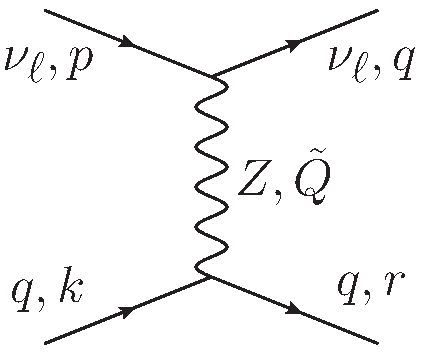
\includegraphics[scale=0.5]{NCprocess_1.pdf}}
\hspace*{0.2\textwidth}
%\label{fig1a}}
\subfloat{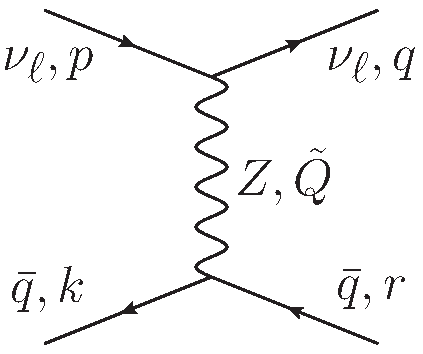
\includegraphics[scale=0.5]{NCprocess_2.pdf}}
%\label{fig1b}}
\caption{Dominant neutral current process diagrams. The left diagram shows the scattering of a neutrino by a given quark $q$ whereas the right diagram depicts the scattering by a given antiquark $q$.}
\label{fig2}
\end{figure}
\end{center}
\par 
The amplitude corresponding to the first diagram is given by
\beq
\label{eq39}
\mathcal{M}(\nu_{\ell}q\to \nu_{\ell}q)=\left(\frac{-ig}{2\cos\theta_W}\right)^2[\bar{u}(q)\gamma_{\mu}\frac{(1-\gamma_5)}{2}u(p)]\frac{-i}{\tilde{Q}^2-M^2_Z}\left(g^{\mu\nu}-\frac{\tilde{Q}^{\mu}\tilde{Q}^{\nu}}{M^2_Z}\right)[\bar{u}(r)\gamma_{\nu}(g_V-g_A\gamma_5)u(k)],
\eeq
where the parameters $g_V$ and $g_A$ are different for up and down quarks,
\beq
\label{eq40}
g^u_V=\frac{1}{2}-\frac{4}{3}\sin^2\theta_W,\,\, g^u_A=\frac{1}{2}
\eeq
and
\beq
\label{eq41}
g^d_V=-\frac{1}{2}+\frac{2}{3}\sin^2\theta_W,\,\, g^d_A=-\frac{1}{2}.
\eeq
By neglecting the term proportional to $\tilde{Q}^{\mu}\tilde{Q}^{\nu}$ we have
\beq
\label{eq42}
\frac{1}{2}\sum_{q \,\tiny{\mathrm{spins}}}|\mathcal{M}(\nu_{\ell}q\to \nu_{\ell}q)|^2=\frac{g^4}{64\cos^4\theta_W(\tilde{Q}^2-M^2_Z)^2}A^{\mu\nu}B_{\mu\nu},
\eeq
where the tensor $A^{\mu\nu}$ is the same already given in Eqs.~(\ref{eq5}) and (\ref{eq6}) for the charged current case and $B_{\mu\nu}$ is written as follows
\beq
\label{eq43}
B_{\mu\nu}=\frac{1}{2}\sum_{q \,\tiny{\mathrm{spins}}}[\bar{u}(r)\gamma_{\mu}(g_V-g_A\gamma_5)u(k)][\bar{u}(k)\gamma_{\nu}(g_V-g_A\gamma_5)u(r)].
\eeq
In Eqs.~(\ref{eq42}) and (\ref{eq43}) we average over the spins of the quark in the initial state and sum over the spins of the quark in the final state. However, in order to simplify the expressions, we include only one sum symbol. By solving the sum in Eq.~\ref{eq43} and disregarding the contribution proportional to $m^2_q$ we obtain
\beq
\label{eq44}
B_{\mu\nu}=2(g^2_V+g^2_A)(r_{\mu}k_{\nu}+r_{\nu}k_{\mu}-(r\cdot k)g_{\mu\nu})-4ig_Vg_A \,r^{\alpha}k^{\beta}\epsilon_{\alpha\beta\mu\nu}.
\eeq
By replacing Eqs.~(\ref{eq7}) and (\ref{eq44}) in Eq.~(\ref{eq42}) we obtain the unpolarized squared amplitude,
\beq
\label{eq45}
|\mathcal{M}|^2_{\mathrm{unpol.}}=\frac{g^4}{2\cos^4\theta_W(Q^2+M^2_Z)^2}\left((g_V+g_A)^2(q\cdot r)(p\cdot k)+(g_V-g_A)^2(q\cdot k)(p\cdot r)\right),
\eeq
that in terms of Madelstam's variables can be written as
\beq
\label{eq46}
|\mathcal{M}|^2_{\mathrm{unpol.}}=\frac{g^4}{8\cos^4\theta_W(Q^2+M^2_Z)^2}\left((g_V+g_A)^2\,\hat{s}^2+(g_V-g_A)^2\,\hat{u}^2\right),
\eeq
where the relations given in Eqs.~(\ref{eq10})-(\ref{eq11}) and (\ref{eq24})-(\ref{eq25}) have been used. By combining this result with the phase space element obtained in Eq.~(\ref{eq17}) we obtain the unpolarized differential cross section,
\beq
\label{eq47}
\frac{d\sigma}{d\hat{t}}(\nu_{\ell}q\to \nu_{\ell}q)=\frac{G^2_F}{4\pi}\frac{M^4_Z}{(Q^2+M^2_Z)^2}\left((g_V+g_A)^2+(g_V-g_A)^2(1-y)^2\right),
\eeq
where the relation in Eq.~(\ref{eq32}) have been used.\par
Let us now compute the right diagram of Fig.~\ref{fig2}. In this case we have
\beq
\label{eq48}
\frac{1}{2}\sum_{q \,\tiny{\mathrm{spins}}}|\mathcal{M}(\nu_{\ell}\bar{q}\to \nu_{\ell}\bar{q})|^2=\frac{g^4}{64\cos^4\theta_W(Q^2+M^2_Z)^2}A^{\mu\nu}\tilde{B}_{\mu\nu},
\eeq
where $A$ is given in Eq.~(\ref{eq7}) and $\tilde{B}$ is defined as
\beq
\label{eq49}
\tilde{B}_{\mu\nu}=\frac{1}{2}\sum_{q \,\tiny{\mathrm{spins}}}[\bar{v}(k)\gamma_{\mu}(g_V-g_A\gamma_5)v(r)][\bar{v}(r)\gamma_{\nu}(g_V-g_A\gamma_5)v(k)],
\eeq
where we have again nelgected the contribution proportional to $\tilde{Q}^{\mu}\tilde{Q}^{\nu}$. By computing the corresponding sum we obtain
\beq
\label{eq50}
\tilde{B}_{\mu\nu}=2(g^2_V+g^2_A)^2(r_{\mu}k_{\nu}+r_{\nu}k_{\mu}-(r\cdot k)g_{\mu\nu})+4ig_Vg_A r^{\alpha}k^{\beta}\epsilon_{\alpha\beta\mu\nu}.
\eeq
By using Eqs.~(\ref{eq7}) and (\ref{eq49}) in Eq.~(\ref{eq48}) we obtain the unpolarized squared amplitude,
\beq
\label{eq51}
|\mathcal{M}|^2_{\mathrm{unpol.}}=\frac{g^4}{8\cos^4\theta_W(Q^2+M^2_Z)^2}\left((g_V-g_A)^2\,\hat{s}^2+(g_V+g_A)^2\,\hat{u}^2\right),
\eeq
from which the unpolalired differential cross section is obtained,
\beq
\label{eq52}
\frac{d\sigma}{d\hat{t}}(\nu_{\ell}\bar{q}\to \nu_{\ell}\bar{q})=\frac{G^2_F}{4\pi}\frac{M^4_Z}{(Q^2+M^2_Z)^2}\left((g_V-g_A)^2+(g_V+g_A)^2(1-y)^2\right).
\eeq
By using Eqs.~(\ref{eq35}) and (\ref{eq52}) along with appropiate parton distribution functions the differential cross section of the process $\nu_{\ell}N\to \nu_{\ell}+\mbox{anything}$ is computed,
\beq
\nonumber
\frac{d^2\sigma}{dxdy}^{\!\!\!(N.C.)}\!\!\!=\frac{G^2_F}{4\pi}\frac{M^4_Z}{(Q^2+M^2_Z)^2}sx \Big\{ \left(f_u(x)L^2_u+f_{\bar{u}}(x)R^2_u+f_d(x)L^2_d+f_{\bar{d}}(x)R^2_d\right) +
\eeq
\beq
\label{eq54}
+\,(1-y)^2\left(f_{\bar{u}}(x)L^2_u+f_u(x)R^2_u+f_{\bar{d}}(x)L^2_d+f_d(x)R^2_d\right) \Big\},
\eeq
where 
\beq
\label{eq55}
L_u\equiv g^u_V+g^u_A = 1-\frac{4}{3}\sin^2\theta_W\,\,
\eeq
\beq
\label{eq56}
\,\,\,L_d\equiv g^d_V+g^d_A = -1+\frac{2}{3}\sin^2\theta_W
\eeq
\beq
\label{eq57}
R_u\equiv g^u_V-g^u_A = -\frac{4}{3}\sin^2\theta_W \,\,\,\,\,\,\,
\eeq
\beq
\label{eq58}
R_d\equiv g^d_V-g^d_A = \frac{2}{3}\sin^2\theta_W\,. \,\,\,\,\,\,\,\,\,
\eeq
We will use te following definitions,
\beq
\label{eq59}
q^0(x)\equiv f_u(x)L^2_u+f_{\bar{u}}(x)R^2_u+f_d(x)L^2_d+f_{\bar{d}}(x)R^2_d,
\eeq
\beq
\label{eq60}
\bar{q}^0(x)\equiv f_{\bar{u}}(x)L^2_u+f_u(x)R^2_u+f_{\bar{d}}(x)L^2_d+f_d(x)R^2_d.
\eeq
If we consider an isoscalar nucleon and take into account the violation of Bjorken scaling we can insert the replacements given in Eqs~.(\ref{eq36})-(\ref{eq37}) into Eqs.~(\ref{eq59}) and (\ref{eq60}) in order to obtain the functions $q^0(x,Q^2)$ and $\bar{q}^0(x,Q^2)$ respectively. Therefore, the differential cross section for the process $\nu_{\ell}N\to \nu_{\ell}+ \mbox{anything}$ with $N=(n+p)/2$ is given by
\beq
\label{eq61}
\frac{d^2\sigma}{dxdy}^{\!\!\!(N.C.)}\!\!\!=\frac{G^2_F}{2\pi}\frac{M^4_Z}{(Q^2+M^2_Z)^2}ME_{\nu}\{ xq^0(x,Q^2)+x\bar{q}^0(x,Q^2)(1-y)^2\}.
\eeq
\section{Computation of the Cross Section - Singlet LQ scenario}
Let us consider a simple scenario in which a LQ with $SU(3)_C\times SU(2)_L\times U(1)_Y$ quantum numbers $(\bf{\bar{3}},\bf{1},\bf{1/3})$ couples to lepton and quarks giving rise to vertices of the type $LQ-l-q$. We will compute the cross section for the s-channel which is the resonant case under the assumption that the LQ couples only to a given family of leptons and a given family of quarks. This assumption goes in the line of \cite{Barger} in which the LQ is assumed to connect the first family of quarks with the third family of leptons (see Eq.~(\ref{eqA13})). Again, we distinguish between a \emph{neutral} (N) and a \emph{charged} (C) case. In the former case there is a neutrino in the final state whereas in the latter there is a cherged lepton. At parton level we have then
$$\mbox{N case: } \nu_{\ell} + D\to \nu_{\ell} + D$$ 
$$\mbox{C case: } \nu_{\ell} + D\to \ell^- + U,$$
where $\ell=e,\mu,\tau$, $U=u,c,t$ and $D=d,s,b$. The corresponding diagrams are depicted in Fig.~\ref{fig3}.
\begin{center}
\begin{figure}[H]
\centering
%\hspace*{-0.4cm}
\subfloat{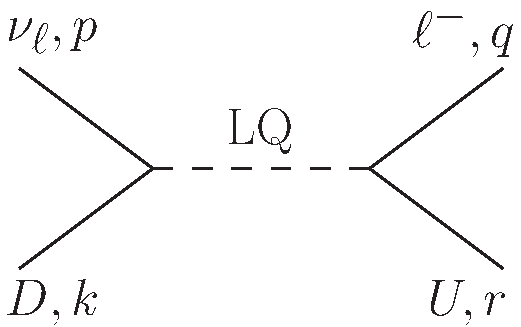
\includegraphics[scale=0.55]{LQ_Cprocess.pdf}}
\hspace*{0.2\textwidth}
%\label{fig1a}}
\subfloat{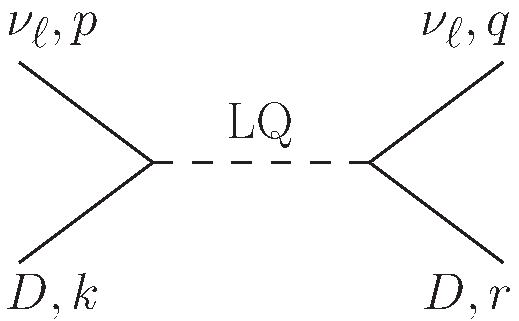
\includegraphics[scale=0.55]{LQ_Nprocess.pdf}}
%\label{fig1b}}
\caption{Relevant s-channel diagrams. The left diagram shows the \emph{charged} process while the right one shows the \emph{neutral} process.}
\label{fig3}
\end{figure}
\end{center}
\par
Let us first compute the cross section corresponding to the C process. The lagrangian is given in Eq.~(\ref{eqA18}) wile the Feynman rules can be derived by using the expansions given in Eqs.~(\ref{eqB1})-(\ref{eqB2}) and (\ref{eqB17})-(\ref{eqB18}). We denote the amplitude corresponding to left-handed (right-handed) particles in the final state as $\mathcal{M}_L(\mathcal{M}_R)$. With this notation the total amplitude is given by
\beq
\label{eq62}
\mathcal{M}=\mathcal{M}_L+\mathcal{M}_R,
\eeq
with
\beq
\label{eq63}
\mathcal{M}_L=g^2_L \frac{[\,\xbar{u}^{\,c}_{DL}(k)u_{\nu L}(p)\,][\,\xbar{u}_{\,\ell L}(q)u^c_{UL}(r)\,]}{(\hat{s}-M^2-iM\Gamma)},
\eeq
\beq
\label{eq64}
\mathcal{M}_R=g_L g_R \frac{[\,\xbar{u}^{\,c}_{DL}(k)u_{\nu L}(p)\,][\,\xbar{u}_{\,\ell R}(q)u^c_{UR}(r)\,]}{(\hat{s}-M^2-iM\Gamma)},
\eeq
where $\hat{s}=(p+k)^2$ and $M$ is the LQ mass. The left-handed contribution can be written as
\beq
\label{eq65}
|\mathcal{M}_L|^2_{\mathrm{unpol.}}\equiv \frac{1}{2}\sum_{\substack{ D,U,\ell \\ \mathrm{spins}}}\frac{g^4_L|a|^2|b|^2}{(\hat{s}-M^2)^2+M^2\Gamma^2},
\eeq
where we have used the following definitions
\beq
\label{eq66}
a\equiv \xbar{u}^{\,c}_{DL}(k)\,u_{\nu L}(p) = \xbar{v}_{DR}(k)\,u_{\nu L}(p),
\eeq
\beq
\label{eq67}
b \equiv \xbar{u}_{\,\ell L}(q)\,u^c_{UL}(r) = \xbar{u}_{\,\ell L}(q)\,v_{UR}(r).
\eeq
In the second equality of Eqs.~(\ref{eq66}) and (\ref{eq67}) we have used the relations in Eqs.~(\ref{eqB15}) and (\ref{eqB16}). From Eq.~(\ref{eq66}) we have
\beq
\label{eq68}
|a|^2 = \mathrm{Tr}\,[\,v_{D}(k)\,\xbar{v}_D(k)u_{\nu L}(p)\,\xbar{u}_{\,\nu L}],
\eeq
and then
\beq
\label{eq69}
\sum_{D \,\mathrm{spins}} |a|^2 = \mathrm{Tr}\,[(\kslash - m_D)P_L\pslash\,\,] = 2(k\cdot p).
\eeq
\par
On the other hand,
\beq
\label{eq70}
|b|^2=\mathrm{Tr}\,[u_{\,\ell}(q)\,\xbar{u}_{\,\ell}(q)\,P_R \,v_U(r)\,\xbar{v}_U(r)\,P_L],
\eeq
and hence
\beq
\label{eq71}
\sum_{U,\ell\,\mathrm{spins}}|b|^2= \mathrm{Tr}\,[\qslash \,(\rslash - m_U)\,P_L]= 2(q\cdot r).
\eeq
We can write these expressions in terms of Mandelstam's variables by taking into account that
$$
\hat{s}=(q+r)^2= m^2_{\ell}+m^2_U +2(q\cdot r)\sim m^2_U + 2(q\cdot r), 
$$
from which we have the relation
\beq
\label{eq72}
2(q\cdot r)=\hat{s}-m^2_U.
\eeq
Similarly,
$$\hat{s}= (p+k)^2=m^2_{\nu}+m^2_D+2(k\cdot p),$$
and neglecting the neutrino and $D$ quark masses we find
\beq
\label{eq73}
2(k\cdot p)=\hat{s}.
\eeq
By using the relations in Eqs.~(\ref{eq72}) and (\ref{eq73}) in Eqs.~(\ref{eq71}) and (\ref{eq69}) respectively we obtain
\beq
\label{eq74}
\sum_{D\,\mathrm{spins}} |a|^2=\hat{s}\quad ,\quad \sum_{U,\ell\,\mathrm{spins}}|b|^2 =\hat{s}-m^2_U,
\eeq
and replacing these expressions into Eq.~(\ref{eq65}) we obtain the following expression
\beq
\label{eq75}
|\mathcal{M}_L|^2_{\mathrm{unpol.}}=\frac{g^4_L}{2}\frac{\hat{s}(\hat{s}-m^2_U)}{(\hat{s}-M^2)^2+M^2\Gamma^2}.
\eeq
\par
Let us turn now to the computation of the right-handed contribution,
\beq
\label{eq76}
|\mathcal{M}_R|^2_{\mathrm{unpol.}}\equiv \frac{1}{2}\sum_{\substack{D,U,\ell \\ \mathrm{spins}}} \frac{g^2_Lg^2_R \,|a|^2 |\tilde{b}|^2}{(\hat{s}-M^2)^2+M^2\Gamma^2},
\eeq
where $a$ was defined in Eq.~(\ref{eq66}) and 
\beq
\label{eq77}
\tilde{b}\equiv \xbar{u}_{\,\ell R}(q)\,u^c_{UR}(r)= \xbar{u}_{\,\ell R}(q)\,v_{UL}(r).
\eeq
From Eq.~(\ref{eq77}) we have
\beq
\label{eq78}
\sum_{U,\ell\, \mathrm{spins}}|\tilde{b}|^2= \mathrm{Tr}\,[\qslash\,(\rslash - m_U)P_R]=2(q\cdot r).
\eeq
By replacing Eqs.~(\ref{eq69}) and (\ref{eq78}) in Eq.~(\ref{eq76}) we obtain
\beq
\label{eq79}
|\mathcal{M}_R|^2_{\mathrm{unpol.}}=\frac{g^2_L g^2_R}{2}\frac{\hat{s}(\hat{s}-m^2_U)}{(\hat{s}-M^2)^2+M^2\Gamma^2}.
\eeq
\par 
The complete unpolarized squared amplitude is given by
\beq
\label{eq80}
|\mathcal{M}|^2_{\mathrm{unpol.}}=|\mathcal{M}_L+\mathcal{M}_R|^2_{\mathrm{unpol.}}=|\mathcal{M}_L| ^2_{\mathrm{unpol.}}+|\mathcal{M}_R|^2_{\mathrm{unpol.}}+2\mathrm{Re}(\mathcal{M}_L\mathcal{M}^*_R)_{\mathrm{unpol.}}.
\eeq
Now we will show that the last term can be neglected and in this sense there is no interference between the left- and right-handed parts of the amplitude. That term is proportional to $|a|^2 b\tilde{b}^*$ with 
\beq
\label{eq81}
b\tilde{b}^* = \mathrm{Tr}\,[u_{\ell}(q)\,\xbar{u}_{\,\ell}(q)\,P_R\,v_U(r)\,\xbar{v}_{\,U}(r)\,P_R],
\eeq
and hence
\beq
\label{eq82}
\frac{1}{2}\sum_{\substack{U, \ell \\ \mathrm{spins}}} b\tilde{b}^*=(1/2)\mathrm{Tr}\,[(\qslash + m_{\ell})\,P_R\,(\rslash - m_U)\,P_R]=-m_{\ell}m_U.
\eeq
We then see that the contribution of the interference term being proportional to the lepton mass is negligible as compared to the other two terms appearing in Eq.~(\ref{eq80}). \par
In order to complete the computation of the cross section it only remains to obtain the LQ width $\Gamma$. We will assume as in \cite{Anchordoqui} that the width is dominated by $LQ \to \ell^+ \bar{U}$ and $LQ \to \bar{\nu}\bar{D}$. Let us call the widths corresponding to these decays as $\Gamma_I$ and $\Gamma_{II}$ respectively. In the case of $\Gamma_I$ we can again compute the left- and right-handed parts separately,
\beq
\label{eq83}
\mathcal{M}^I_L= ig_L[\,\xbar{v}^{\,c}_{\,UL}(p_2)\,v_{\ell L}(p_1)]
\eeq
\beq
\label{eq84}
\mathcal{M}^{I}_R= ig_R[\,\xbar{v}^{\,c}_{\,UR}(p_2)\,v_{\ell R}(p_1)].
\eeq
From Eqs.~(\ref{eq83}) and (\ref{eq84}) we obtain
\beq
\label{eq85}
|\mathcal{M}^I_L|^2_{\mathrm{unpol.}}=2 g^2_L (p_1\cdot p_2)=g^2_L(M^2-m^2_U)
\eeq
\beq
\label{eq86}
|\mathcal{M}^I_R|^2_{\mathrm{unpol.}}=2 g^2_R (p_1\cdot p_2)=g^2_R(M^2-m^2_U).
\eeq
The differential width is given by
\beq
\label{eq87}
d\Gamma_I=\frac{1}{32\pi^2}|\mathcal{M}^I|^2\frac{|\vec{p}_1|}{M^2}d\Omega_1=\frac{1}{32\pi^2}(g^2_L+g^2_R)\frac{M^2-m^2_U}{M^2}\frac{M^2-m^2_U}{2M}d\phi_1\,d(\cos\theta_1),
\eeq
where we have used that $|\vec{p}_1|=(M^2-m^2_U)/2M$ if the lepton mass is neglected. By performing the integrations we obtain
\beq
\label{eq88}
\Gamma_1=\frac{M}{16\pi}(g^2_L+g^2_R)\left(1-\frac{m^2_U}{M^2}\right)^2.
\eeq
Let us now compute $\Gamma_2$. The corresponding amplitude is given by
\beq
\label{eq89}
\mathcal{M}^{II}=-ig_L\,[\xbar{v}^{\,c}_{DL}(p_2)\,v_{\nu L}(p_1)],
\eeq
from which we obtain
\beq
\label{eq90}
|\mathcal{M}^{II}|^2_{\mathrm{unpol.}}=2 g^2_L (p_1\cdot p_2)=g^2_L M^2.
\eeq
Therefore, the differential width is
\beq
\label{eq91}
d\Gamma_{II}=\frac{1}{32\pi^2}(g^2_L+g^2_R)\frac{(M^2-m^2_U)}{M^2}\frac{(M^2-m^2_U)}{2M}\,d\phi_1d(\cos\theta_1),
\eeq
where we have use that $|\vec{p}_1|=M/2$ under the assumption $m^2_{\nu},m^2_{\ell}\simeq 0$. By integrating Eq.~(\ref{eq91}) over the angles we have
\beq
\label{eq92}
\Gamma_{II}=\frac{M}{16\pi}g^2_L.
\eeq
From Eqs.~(\ref{eq88}) and (\ref{eq92}) we see that the LQ width is given by
\beq
\label{eq93}
\Gamma = \frac{M}{16\pi}\left\{ g^2_L [(1-\lambda_U)^2+1]+g^2_R(1-\lambda_U)^2 \right\},
\eeq
where $\lambda_U\equiv m^2_U/M^2$. \par
By using Eq.~(\ref{eq93}) and under the narrow-width approximation,
\beq
\label{eq94}
\frac{1}{(\hat{s}-M^2)^2+M^2\Gamma^2}\approx \frac{\pi}{M\Gamma}\delta (\hat{s}-M^2),
\eeq
we obtain from Eqs.~(\ref{eq75}) and (\ref{eq79}) that
\beq
\label{eq95}
|\mathcal{M}(\nu D \to \ell^{-}U)|^2_{\mathrm{unpol.}}=\frac{8\pi^2 g^2_L (g^2_L+g^2_R)\hat{s}(\hat{s}-m^2_U)}{M^2[(g^2_L+g^2_R)(1-\lambda_U)^2+g^2_L]}\delta (\hat{s}-M^2).
\eeq
From Eq.~(\ref{eq95}) we can write the corresponding unpolarized differential cross section for the C case:
\beq
\label{eq96}
\frac{d\sigma}{d\hat{t}}^{C}=\frac{\pi}{2\hat{s}}\frac{g^2_L (g^2_L+g^2_R)(\hat{s}-m^2_U)}{M^2[(g^2_L+g^2_R)(1-\lambda_U)^2+g^2_L]}\delta (\hat{s}-M^2).
\eeq
Now we can write the differential cross section for the process $\nu N\to \ell^{-} + \mbox{anything}$:
\beq
\label{eq97}
\frac{\,\,d\sigma^C}{dQ^2 dx}=\frac{\pi}{2xs}\frac{g^2_L (g^2_L+g^2_R)(xs-m^2_U)}{M^2[(g^2_L+g^2_R)(1-\lambda_U)^2+g^2_L]}f_D(x)\delta (xs-M^2),
\eeq
where $f_D(x)$ is the parton distribution function corresponding to the down-type quark $D$ in the nucleon $N$. In order to use the inelasticity parameter we have to obtain the relation between $Q^2$ and $x$ in the case in which the mass of the quark in the final state is not neglected and then it is still valid in the case of considering the top quark. The mass of the up quark can be related to the longitudinal fraction $\xi$ as follows
\beq
\label{eq98}
m^2_U = r^2 = (p+k-q)^2=(\tilde{Q}+k)^2=\tilde{Q}^2+2\tilde{Q}\cdot k = -Q^2 +2\xi P\cdot\tilde{Q},
\eeq
from which
\beq
\label{eq99}
\xi=x, \mbox{ with } x \equiv \frac{Q^2+m^2_U}{2 P\cdot \tilde{Q}}.
\eeq
The inelasticity parameter can be writen in turn in the following manner
\beq
\label{eq100}
y=\frac{2 P\cdot \tilde{Q}}{2P\cdot p}=\frac{2P\cdot \tilde{Q}}{2M_N E_{\nu}}.
\eeq
From Eqs.~(\ref{eq99}) and (\ref{eq100}),
\beq
\label{eq101}
Q^2=xy(2M_N E_{\nu})-m^2_U, \,\mbox{ and }\, dx\,dQ^2 = x(2M_N E_{\nu}) dx dy.
\eeq
By using Eqs.~(\ref{eq97}) and (\ref{eq101}) and integrating in $x$ we finally obtain
\beq
\label{eq102}
\frac{d\sigma}{dy}^C =\frac{\pi}{2}\frac{g^2_L(g^2_L+g^2_R)(1-\lambda_U)}{(g^2_L+g^2_R)(1-\lambda_U)^2+g^2_L}\frac{f_D(M^2/s)}{s},
\eeq
where the $1/s$ factor arises from the integration by using the delta function $\delta (xs-M^2)$. We also note that the delta function imposes $x=M^2/s$, so that
\beq
\label{eq103}
Q^2 = M^2 y -m^2_U,
\eeq
and hence $\lambda_U \leqslant y \lesssim 1 $. 
Let us now to compute the cross section for the neutral case. The amplitude is given by
\beq
\label{eq104}
\mathcal{M}= (ig_L)^2 \frac{[\xbar{u}^{\,c}_{DL}(k)\,u_{\nu L}(p)][\xbar{u}_{\nu L}(q)\,u^c_{DL}(r)]}{\hat{s}-M^2-iM\Gamma}.
\eeq 
The unpolarized squared amplitude is
\beq
\label{eq105}
|\mathcal{M}|^2_{\mathrm{unpol.}}\equiv \frac{1}{2}\sum_{D\,\mathrm{spins}}\frac{g^4_L |a|^2|c|^2}{(\hat{s}-M^2)^2+M^2\Gamma^2},
\eeq
where $a$ was already defined and
\beq
\label{eq106}
c\equiv \xbar{u}_{\nu L}(q)\,v_{DR}(r).
\eeq
From Eq.~(\ref{eq106}) we have
\beq
\label{eq107}
\sum_{D \,\mathrm{spins}}|c|^2= \mathrm{Tr}\,[\,(\qslash + m_{\nu})\,P_R\,(\rslash - m_D)\,P_L]=2(q\cdot r)=\hat{s}.
\eeq
By using this expression we obtain
\beq
\label{eq108}
|\mathcal{M}|^2_{\mathrm{unpol.}}=\frac{\pi g^4_L}{M\Gamma} \frac{\hat{s}^2}{2}\delta (\hat{s}-M^2),
\eeq
where we have used again the narrow-width approximation. The differential cross section is then given by
\beq
\label{eq109}
\frac{d\sigma}{d\hat{t}}^N =\frac{\pi g^4_L \delta (\hat{s}-M^2)}{2M^2[(g^2_L+g^2_R)(1-\lambda_U)^2+g^2_L]}.
\eeq
From this equation we can derive the differential cross section for the process $\nu N \to \nu + \mbox{anything}$,
\beq
\label{eq110}
\frac{d\sigma^N}{dy}=\frac{\pi}{2}\frac{g^4_L}{(g^2_L+g^2_R)(1-\lambda_U)^2+g^2_L}\frac{f_D(M^2/s)}{s},
\eeq
where we have performed the integration over $x$. We note that in this case $Q^2=xys$ and since the delta function imposes $x=M^2/s$, $Q^2=yM^2$, restoring the range of the inelasticity parameter, $0\leqslant y \leqslant 1$.
%%%%%%%%%%%%%%%%%%%%%%%%%%%%%%%%%%%%%%
\section{Computation of the Cross Section - Triplet LQ scenario}
\beq
\mathcal{M}_1=-\frac{\lambda^{i*}_{\ell}\lambda^j_{\ell^{\prime}}}{D(\chi_1;p+k)}[\,\xbar{v}_R(\nu_{\ell};p)\,u_L(U_i;k)\,][\,\xbar{u}_L(U_j;r)\,v_R(\nu_{\ell^{\prime}};q)\,]
\eeq
\beq
\mathcal{M}_2=-\frac{\lambda^{i*}_{\ell}\lambda^j_{\ell^{\prime}}}{2 D(\chi_2;p+k)}[\,\xbar{v}_R(\nu_{\ell};p)\,u_L(D_i;k)\,][\,\xbar{u}_L(D_j;r)\,v_R(\nu_{\ell^{\prime}};q)\,]
\eeq
\beq
\mathcal{M}_3=-\frac{\lambda^{j*}_{\ell}\lambda^i_{\ell^{\prime}}}{2 D(\chi_1;p-r)}[\,\xbar{v}_R(\nu_{\ell};p)\,v_L(\xbar{U}_j;r)\,][\,\xbar{v}_L(\xbar{U}_i;k)\,v_R(\nu_{\ell^{\prime}};q)\,]
\eeq
\beq
\mathcal{M}_4=-\frac{\lambda^{j*}_{\ell}\lambda^i_{\ell^{\prime}}}{2 D(\chi_2;p-r)}[\,\xbar{v}_R(\nu_{\ell};p)\,v_L(\xbar{D}_j;r)\,][\,\xbar{v}_L(\xbar{D}_i;k)\,v_R(\nu_{\ell^{\prime}};q)\,]
\eeq
%%%%%%%%%%%%%%%%%%%%%%%%
\beq
|\mathcal{M}_1|^2_{\mathrm{unpol.}}=\frac{|\lambda^{i}_{\ell}\lambda^j_{\ell^{\prime}}|^2}{2|D(\chi_1;p+k)|^2}\hat{s}\,(\hat{s}-m^2_{U_j}) 
\eeq
%%%%%%%%%%%%%%%%%%%%%%%%%%%%%%%%%%%%%%
\appendix
\section{Electroweak-singlet LQ Lagrangian}
\label{ap1}
Let us assume the case of a leptoquark $S$ whose $SU(3)_C\times SU(2)_L\times U(1)_Y$ quantum numbers are $(\bf{\bar{3}},\bf{1},\bf{1/3})$. In order to construct a gauge and Lorentz invariant lagrangian that describe the interaction of this LQ with quark and leptons, the transformation properties of the involved fields must be taken into account. Here, we will focus on the gauge group $SU(2)_L\times U(1)_Y$ and the Lorentz transformation. The fields along with their number quantums are given in the following equation
\beq
\nonumber
Q_L=
\begin{pmatrix}
u_L \\
d_L \\
\end{pmatrix}
\to (\mathbf{2},\mathbf{1/6}),\,\,
L_L=
\begin{pmatrix}
\nu_L \\
\ell_L \\
\end{pmatrix}
\to (\mathbf{2},\mathbf{-1/2}),
\eeq
\beq
\label{eqA1}
u_R \to (\mathbf{1},\mathbf{2/3}),\,\,
d_R \to (\mathbf{1},\mathbf{-1/3}),\,\, \ell_R \to (\mathbf{1},\mathbf{-1}).
% \to (\mathbf{1},\mathbf{-1}).
\eeq
If the fields $S$ and $L_L$ are included in a given term, then one would say that the field $\xbar{Q}_L$ must also be included in order to satisfy $SU(2)_L$ gauge invariance. However, the net hypercharge in the term $\xbar{Q}_L L_L S$ would not be zero: $-1/6-1/2+1/3 \neq 0$. Hence, we need a doublet that transforms as $\xbar{Q}_L$ under $SU(2)_L$ and as $Q_L$ under $U(1)_Y$. The requirement on $Y$ is easily satisfied by taking $\xbar{Q}^{\dagger}_L$. But unfortunately this field does not transform as $\xbar{Q}_L$ under $SU(2)_L$. Hence, we will use $\xbar{Q}^{\dagger}_L$ but adjusting it to obtain the appropiate transformation property. We will show now that the field $$\widetilde{\xbar{Q}}_L\equiv -i(\tau_2\, \xbar{Q}^{\dagger}_L)^{T}$$ transforms as $\xbar{Q}_L$ under $SU(2)_L$. Under an infinitesimal transformation we have
\beq
\label{eqA2}
\delta\, \xbar{Q}_L = -\frac{i}{2}g\, \omega_j \,\xbar{Q}_L \tau_j,
\eeq
from which 
\beq
\label{eqA3}
\delta \,\xbar{Q}^{\dagger}_L = \frac{i}{2}g\, \omega_j\tau_j\, \xbar{Q}^{\dagger}_L.
\eeq
From Eq.~(\ref{eqA3}) and the definition of $\widetilde{\xbar{Q}}_L$ we can write
\beq
\nonumber
\delta\, \widetilde{\xbar{Q}}_L = -i\left( \tau_2\, \frac{i}{2}\,g\,\omega_j \tau_j\, \xbar{Q}^{\dagger}_L\right)^{T}
\eeq
\beq
\nonumber
\qquad\quad= -i\left(-\frac{i}{2}\,g\,\omega_j\tau^T_j\tau_2\,\xbar{Q}^{\dagger}_L \right)^{T}
\eeq
\beq
\nonumber
\qquad=-\frac{i}{2}\,g\,\omega_j(-i\tau_2\,\xbar{Q}^{\dagger}_L)^T\tau_j
\eeq
\beq
\label{eqA4}
=-\frac{i}{2}\,g\,\omega_j\, \widetilde{\xbar{Q}}_L\, \tau_j,\quad
\eeq
where we have used that $\tau_2\tau_j = -\tau^T_j\tau_2$. By comparing Eqs.~(\ref{eqA2}) and (\ref{eqA4}) we see that $\widetilde{\xbar{Q}}_L =-i(\tau_2\,\xbar{Q}^{\dagger}_L)^T=\xbar{Q}^{*}_L \,i\tau_2$ transforms as $\xbar{Q}_L$ under $SU(2)_L$. Also, $\widetilde{\xbar{Q}}_L$ transforms as $Q_L$ under $U(1)_Y$ as can be easily checked from its definition. However, if we were to write the interaction as $\widetilde{\xbar{Q}}_L L_L S= \xbar{Q}^*_Li\tau_2 L_L S$ then the couplings between the fields with $s=1/2$ would be of the form $\xbar{\psi}^* \psi$ which is not Lorentz invariant in contrast to $\xbar{\psi}\psi$. The Lorentz invariance can be restorted if the charge conjugate field is used since $\xbar{\psi}^c \psi$ with $\xbar{\psi}^c\equiv -i\psi^T \gamma^2\gamma^0$ is invariant as we will show in the following. \par
Under an infinitesimal Lorentz transformation,
\beq
\label{eqA5}
\psi \to \Lambda_{1/2}\,\psi= \left(1-\frac{i}{2}\omega_{\mu\nu}S^{\mu\nu}\right)\psi,
\eeq
where $S^{\mu\nu}=i[\gamma^{\mu},\gamma^{\nu}]/2$. On the other hand, the charge conjugate field transforms as follows
\beq
\label{eqA6}
\xbar{\psi}^c=-i\psi^T \gamma^2\gamma^0 \to -i\left[\left(1-\frac{i}{2}\omega_{\mu\nu}S^{\mu\nu}\right)\psi\right]^T \gamma^2\gamma^0=-i\psi^T\left(1-\frac{i}{2}\omega_{\mu\nu}S^{\mu\nu\,T}\right)\gamma^2\gamma^0. 
\eeq
From the definition of $S^{\mu\nu}$ it can be shown that $S^{0i\, T}=S^{0i}$ if $i=1,3$ and $S^{02\, T}=-S^{02}$ whereas $S^{ij\, T}=S^{ij}$ if $i=2$ or $j=2$ and $S^{ij\, T}=-S^{ij}$ otherwise. Moreover, it is easy to show that 
\begin{itemize}
\item $[S^{\mu\nu},\gamma^2]=0$ if $\mu\neq 2$ and $\nu\neq 2$ and $\{S^{\mu\nu},\gamma^2\}=0$ otherwise.
\item $[S^{\mu\nu},\gamma^0]=0$ if $\mu\neq 0$ and $\nu\neq 0$ and $\{S^{\mu\nu},\gamma^0\}=0$ otherwise.
\end{itemize}
From these properties we see that $S^{\mu\nu\,T}\gamma^2\gamma^0=-\gamma^2\gamma^0 S^{\mu\nu}$ and finally arrive to 
\beq
\label{eqA7}
\xbar{\psi}^c\to -i\psi^T\gamma^2\gamma^0\left(1+\frac{i}{2}\omega_{\mu\nu}S^{\mu\nu}\right)=\xbar{\psi}^c \Lambda^{-1}_{1/2}.
\eeq
By combining Eqs.~(\ref{eqA5}) and (\ref{eqA7}) we arrive to the result that $\xbar{\psi}^c \psi$ is invariant under Lorentz transformations. In Eq.~(\ref{eqA4}) we have proved that the transformation law under $SU(2)_L$ of $\xbar{Q}^{\,*}_L i\tau_2$ and $\xbar{Q}_L$ is the same but we have also shown that in order to get Lorentz invariant interactions the field $\xbar{Q}^{\,c}_L\equiv -i Q^T_L \gamma^2\gamma^0$ must be used instead of $\xbar{Q}^{\,*}_L$. Hence, we should prove that $\xbar{Q}^{\,c}_L i\tau_2$ also transforms as $\xbar{Q}_L$ under $SU(2)_L$. \par
First we note that in general $\xbar{\psi}^*=(\psi^{\dagger}\gamma^0)^*=\psi^T \gamma^0$ and then
$$\xbar{\psi}^c=-i\psi^T \gamma^2\gamma^0=-i\xbar{\psi}^*\gamma^0\gamma^2\gamma^0=\xbar{\psi}^* i\gamma^2.$$
In this way we can obtain $\xbar{Q}^{\,c}_L$ from $\xbar{Q}^{\,*}_L$ as follows
\beq
\label{eqA8}
\xbar{Q}^{\,c}_L=\xbar{Q}^{\,*}_L\,(i\gamma^2 \mathds{1}_{SU(2)_L})
\eeq
and then
\beq
\label{eqA9}
\xbar{Q}^{\,c}_L i\tau_2 = \xbar{Q}^{\, *}_L\,i\gamma^2 \mathds{1}_{SU(2)_L} i\tau_2
= \xbar{Q}^{\, *}_L i\tau_2\, i\gamma^2 \mathds{1}_{SU(2)_L}=\widetilde{\xbar{Q}}_L i\gamma^2 \mathds{1}_{SU(2)_L}.
\vspace*{2mm}
\eeq
From Eqs.~(\ref{eqA9}) and (\ref{eqA4}) we can derive the required transformation law,
\beq
\nonumber
\delta (\xbar{Q}^{\,c}_L i\tau_2)=\delta \widetilde{\xbar{Q}}_L \,i\gamma^2 \mathds{1}_{SU(2)_L}
\eeq
\beq
\nonumber
\qquad\qquad\qquad\quad\,\,\, = -\frac{i}{2}g\,\omega_j\, \widetilde{\xbar{Q}}_L\, \tau_j\,i\gamma^2 \mathds{1}_{SU(2)_L}
\eeq
\beq
\label{eqA10}
\qquad\qquad\quad = -\frac{i}{2}g\,\omega_j\, (\xbar{Q}^{\,c}_L i\tau_2)\tau_j.
\eeq
From Eqs.~(\ref{eqA10}) and (\ref{eqA2}) we see that $\xbar{Q}^{\,c}_L i\tau_2$ transforms as $\xbar{Q}_L$ under $SU(2)_L$. Also, from Eq.~(\ref{eqA8}) it transforms as $Q_L$ under $U(1)_Y$. Therefore, we conclude that the interaction $\xbar{Q}^{\,c}_L i\tau_2\,L_L S$ is $SU(2)_L\times U(1)_Y$ invariant and also Lorentz invariant. \par
The case of right-handed fields is easier since they are all $SU(2)_L$ singlets and hence we need to be careful only with the $U(1)_Y$ and Lorentz invariance. By taking into account the discussion given above, we can conclude that the suitable interaction is $\xbar{u}^{\,c}_R \ell_R S$. On one hand, the hypercharge of this term is $2/3-1+1/3=0$ and on the other hand, the presence of the charge conjugate field $\xbar{u}^{\,c}_R$ guarantees the Lorentz invariance.
We are now ready to write down the the terms of the LQ lagrangian that describe the interaction between quarks and leptons. If we consider only one LQ mediating the lepton-quark interaction, these terms are written as follows,
\beq
\label{eqA11}
\mathcal{L}_{LQ}\supset g^L_{ij}\,\,\xbar{Q}^{\,c}_{iL}i\tau_2 L_{jL} S + g^R_{ij}\,\,\xbar{u}^{\,c}_{iR}\,\ell_{jR}\,S + \mathrm{h.c.},
\eeq  
where the indices $i$ and $j$ denote the quark and lepton families respectively and the sum over them is implicit. This form is adopted for example in \cite{Dutta}. Conversely, in the case of assuming no mixing between the families, universal couplings and one LQ by family, we would have
\beq
\label{eqA12}
\mathcal{L}_{LQ}\supset (g^L\,\,\xbar{Q}^{\,c}_{iL}i\tau_2 L_{iL} +g^R\,\,\xbar{u}^{\,c}_{iR}\,\ell_{iR})S_i + \mathrm{h.c.}
\eeq
This form is used for example in \cite{Anchordoqui}. Finally, in the case assumed in \cite{Barger}, in which the LQ couples only to the first family of quarks and the third family of leptons, we have
\beq
\label{eqA13}
\mathcal{L}_{LQ}\supset (g^L\, \xbar{Q}^{\,c}_{1L}i\tau_2 L_{3L} + g^R\, \xbar{u}^{\,c}_{1R}\,\ell_{3R})S + \mathrm{h.c.},
\eeq 
where $Q_{1L}= (u,d)^T$, $L_{3L}=(\nu_{\tau L}, \tau_L)^T$, $u_{1R}=u_R$ and $\ell_{3R}=\tau_R$.
It is instructive to expand a generic term and compute the corresponding hermitian conjugate,
\beq
\label{eqA14}
\xbar{Q}^{\,c}_{L}i\tau_2 L_{L} S = (\xbar{u}^{\,c}_L\,\ell_L-\xbar{d}^{\,\,c}_L\,\nu_L)S,
\eeq
%
\beq
\label{eqA15}
(\xbar{u}^{\,c}_L\,\ell_L S)^{\dagger}=S^{\dagger}\ell^{\dagger}_L (\xbar{u}^{\,c}_L)^{\dagger}=
S^{\dagger}\,\xbar{\ell}_L \gamma^0 \left((-i\gamma^2 u_L)^T\gamma^0 \right)^{\dagger}=
S^{\dagger}\,\xbar{\ell}_L (-i\gamma^2 u_L)^*=S^{\dagger}\,\xbar{\ell}_L (-i\gamma^2 u^*_L)= S^{\dagger}\,\xbar{\ell}_L u^c_L.
\eeq
Similarly, it can be shown that
\beq
\label{eqA16}
(\xbar{d}^{\,\,c}_L \nu_L S)^{\dagger}=S^{\dagger}\xbar{\nu}_L d^{\,c}_L,
\eeq
\beq
\label{eqA17}
(\xbar{u}^{\,c}_R\,\ell_R S)^{\dagger}=S^{\dagger}\xbar{\ell}_R\,u^c_R.
\eeq
By using Eqs.~(\ref{eqA14})-(\ref{eqA17}) we can write the lagrangian that describes the interaction between a given family of quarks and a given family of leptons in the following manner,
\beq
\label{eqA18}
\mathcal{L}=g_L\,\left\{(\xbar{u}^{\,c}_L\ell_L - \xbar{d}^{\,\,c}_L\nu_L)S + S^{\dagger}(\xbar{\ell}_L u^{c}_L - \xbar{\nu}_Ld^{\,c}_L) \right\} + g_R\,\left\{\xbar{u}^{\,c}_R\ell_R S + S^{\dagger}\,\xbar{\ell}_R u^c_R \right\},
\eeq
where we have assumed that the couplings $g_{L,R}$ are real. This lagrangian is the one that must be taken into account in order to compute a generic s-channel diagram with the LQ as mediator.
\section{How to use Conjugate Fields}
\label{ap2}
The fields describing a $s=1/2$ fermion can be written as follows
\beq
\label{eqB1}
\psi(x) = \int \frac{d^3p}{(2\pi)^3}\frac{1}{\sqrt{2E_{\mathbf{p}}}}\sum_s (a^s_{\mathbf{p}}\,u^s(p)e^{-ipx} + b^{s\dagger}_{\mathbf{p}}\,v^s(p)e^{ipx}),
\eeq
\beq
\label{eqB2}
\xbar{\psi}(x)= \int \frac{d^3p}{(2\pi)^3}\frac{1}{\sqrt{2E_{\mathbf{p}}}}\sum_s (b^s_{\mathbf{p}}\,\xbar{v}^{\,s}(p)e^{-ipx}+a^{s\dagger}_{\mathbf{p}}\,\xbar{u}^{\,s}(p)e^{ipx}).
\eeq
Under the action of the charge conjugation operator $C$, we have
\beq
\label{eqB3}
C\psi(x)C = \int \frac{d^3p}{(2\pi)^3}\frac{1}{\sqrt{2E_{\mathbf{p}}}}\sum_s (b^s_{\mathbf{p}}\,u^s(p)e^{-ipx} + a^{s\dagger}_{\mathbf{p}}\,v^s(p)e^{ipx}),
\eeq
\beq
\label{eqB4}
C\xbar{\psi}(x)C=  \int \frac{d^3p}{(2\pi)^3}\frac{1}{\sqrt{2E_{\mathbf{p}}}}\sum_s (a^s_{\mathbf{p}}\,\xbar{v}^{\,s}(p)e^{-ipx}+b^{s\dagger}_{\mathbf{p}}\,\xbar{u}^{\,s}(p)e^{ipx}).
\eeq
From Eqs.~(\ref{eqB3}) and (\ref{eqB4}) it can be shown that
\beq
\label{eqB5}
C\psi(x)C = -i\gamma^2 \psi^* \equiv \psi^c,
\eeq
\beq
\label{eqB6}
C\xbar{\psi}(x)C= (-i\gamma^2\psi)^T\gamma^0\equiv \xbar{\psi}^{\,c}.
\eeq
Let us extend these definitions to the spinors, so that we have
\beq
\label{eqB7}
u^s(p)^c \equiv -i \gamma^2 u^s(p)^* = v^s(p),
\eeq
\beq
\label{eqB8}
v^s(p)^c \equiv -i \gamma^2 v^s(p)^* = u^s(p),
\eeq
\beq
\label{eqB9}
\xbar{u}^{\,s}(p)^c \equiv (-i\gamma^2 u(p))^T \gamma^0 =[(-i\gamma^2 u(p)^*)^*]^T \gamma^0 = \xbar{v}^{\,s}(p),
\eeq
\beq
\label{eqB10}
\xbar{v}^{\,s}(p)^c \equiv (-i\gamma^2 v(p))^T \gamma^0 = \xbar{u}^{\,s}(p).
\eeq
By using these definitions along with Eqs.~(\ref{eqB3})-(\ref{eqB6}) we can write,
\beq
\label{eqB11}
\psi^c =\int \frac{d^3p}{(2\pi)^3}\frac{1}{\sqrt{2E_{\mathbf{p}}}}\sum_s (b^s_{\mathbf{p}}\,v^s(p)^c \,e^{-ipx} + a^{s\dagger}_{\mathbf{p}}\,u^s(p)^c\, e^{ipx}),
\eeq
\beq
\label{eqB12}
\xbar{\psi}^{\,c} = \int \frac{d^3p}{(2\pi)^3}\frac{1}{\sqrt{2E_{\mathbf{p}}}}\sum_s (a^s_{\mathbf{p}}\,\xbar{u}^{\,s}(p)^c \,e^{-ipx}+b^{s\dagger}_{\mathbf{p}}\,\xbar{v}^{\,s}(p)^c\, e^{ipx}).
\eeq
Regarding the left- and right-handed fields, we will use the same definitions given in Eqs.~(\ref{eqB5})-(\ref{eqB6}),
\beq
\label{eqB13}
\psi^c_{L,R} = -i\gamma^2 (\psi_{L,R})^* = P_{R,L} \psi^c,
\eeq
\beq
\label{eqB14}
\xbar{\psi}^{\,c}_{L,R} = (-i\gamma^2 \psi_{L,R})^T \gamma^0 = \xbar{\psi}^{\,c} P_{L,R},
\eeq
where $P_{R,L}=(1\pm \gamma^5)/2$. Similarly, by applying the definitions in Eqs.~(\ref{eqB7})-(\ref{eqB10}) to the left- and right-handed spinors we obtain
\beq
\label{eqB15}
u^c_{L,R}= v_{R,L}\,, \qquad \xbar{u}^{\,c}_{L,R}= \xbar{v}_{R,L}\,,
\eeq
\beq
\label{eqB16}
v^c_{L,R}= u_{R,L}\,, \qquad \xbar{v}^{\,c}_{L,R}= \xbar{u}_{R,L}.
\eeq
By combining the expansions in Eqs.~(\ref{eqB3}) and (\ref{eqB4}) with Eqs.~(\ref{eqB13}) and (\ref{eqB14}) and the relations in Eqs.~(\ref{eqB15}) and (\ref{eqB16}) we arrive to the following expansions
\beq
\label{eqB17}
\psi^c_{L,R} =\int \frac{d^3p}{(2\pi)^3}\frac{1}{\sqrt{2E_{\mathbf{p}}}}\sum_s (b^s_{\mathbf{p}}\,v^s_{L,R}(p)^c \,e^{-ipx} + a^{s\dagger}_{\mathbf{p}}\,u_{L,R}^s(p)^c\, e^{ipx}),
\eeq

\beq
\label{eqB18}
\xbar{\psi}^{\,c}_{L,R} = \int \frac{d^3p}{(2\pi)^3}\frac{1}{\sqrt{2E_{\mathbf{p}}}}\sum_s (a^s_{\mathbf{p}}\,\xbar{u}^{\,s}_{L,R}(p)^c \,e^{-ipx}+b^{s\dagger}_{\mathbf{p}}\,\xbar{v}^{\,s}_{L,R}(p)^c\, e^{ipx}).
\eeq
In the case of the fields $\psi^c$ and $\xbar{\psi}^{\,c}$ the expansions in Eqs.~(\ref{eqB11}) and (\ref{eqB12}) must be used and the relations in Eqs.~(\ref{eqB7})-(\ref{eqB10}) allow to replace the charge conjugate spinors by the {\em usual} spinors. On the other hand, in the case of the fields $\psi^c_{L,R}$ and $\xbar{\psi}^{\,c}_{L,R}$ we must take the expansions in Eqs.~(\ref{eqB17}) and (\ref{eqB18}) along with the relations in Eqs.~(\ref{eqB15}) and (\ref{eqB16}). 
%%%%%%%%%%%%%%%%%%%%%%%%%%%%%%%%%%%%%%%%%%
\section{Electroweak-triplet LQ Lagrangian}
\label{ap3}
Let us review how to represent a $SU(2)$ triplet in terms of a $2\times 2$ matrix $\chi$ which transforms under the group as follows,
\beq
\label{eqC1}
\chi \to U \chi U^{\dagger},
\eeq 
where $U= \exp(i\omega _j\tau_j/2)$ and $\tau_j$ is the $j$-th Pauli matrix. In the spin one representation of $SU(2)$, the basis of the representation space is given by eigenvectors of both $J^2$ and $J_3$. Hence, in that basis the generator is diagonal with eigenvalues $-1,0,1$. The so called triplet is given by a column vector,
\beq
\label{eqC2}
\chi=
\begin{pmatrix}
\chi_1 \\
\chi_2 \\
\chi_3
\end{pmatrix},
\eeq 
where $\chi_1$ have $J_3$ quantum number $+1$, $\chi_2$ has $0$ and $\chi_3$ has $-1$. In order to express this triplet as a matrix we need to represent the state $\chi_i$ by a matrix $M_i$ that is the analog of an eigenstate of $J_3$. This condition is written as follows,
\beq
\label{eqC3}
[J_3,M_i]=\lambda_i M_i,
\eeq
where $\lambda_i=1,0,-1$ for $i=1,2,3$ respectively. On the other hand, the transformation law given in Eq.~(\ref{eqC1}) is obviously valid in the case of the representation $\mathbf{2}\otimes \mathbf{\bar{2}}$. By using tensorial notation, this representation is written as $T^i_{\,j}$, which can be splitted into two tensors that are invariant under the transformation law in Eq.~(\ref{eqC1}), one is traceless and the other is proportional to the identity. This is nothing but the decomposition of the direct product representation into a direct sum, $\mathbf{2}\otimes \mathbf{\bar{2}}=\mathbf{3}\oplus\mathbf{1}$ or in tensorial notation $T^i_{\,j}=A^i_{\,j}+B\delta^i_{\,j}$, where $A^i_{\,j}$ is traceless. This tensor can then be used to represent the triplet. We need to consider $2\times 2$ traceless matrices that fulfill Eq.~(\ref{eqC3}) with $J_3=\tau_2/2$. The Pauli matrices are in fact traceless and can be chosen as a basis of the space of $2\times 2$ traceless matrices,
\beq
\label{eqC4}
M_i=\sum^3_{i=1} c_{ij}J_j,
\eeq
where $J_j=\tau_j/2$. By replacing Eq.~(\ref{eqC4}) in Eq.~(\ref{eqC3}), we obtain
\beq
\label{eqC5}
M_1=c_1(J_1+iJ_2)\, ,\quad M_2=c_2 J_3\, , \quad M_3=c_3(J_1-iJ_2), 
\eeq
and hence the triplet can be written as follows,
\beq
\label{eqC6}
\chi=\chi_1 M_1 + \chi_2 M_2 + \chi_3 M_3.
\eeq
By choosing the normalization $c_1=c_3=1$ and $c_2=1/\sqrt{2}$ we get
\beq
\label{eqC7}
\chi =
\begin{pmatrix}
\chi_2/\sqrt{2} & \chi_1 \\
\chi_3 & -\chi_2/\sqrt{2} \\
\end{pmatrix}
.
\eeq
We note that if we assign the hypercharge $-1/3$ to the triplet, the electric charges of the scalars $\chi_{1,2,3}$ are respectively $2/3,-1/3$ and $-4/3$. Now that we have the matrix representation (Eq.~(\ref{eqC7}))of the triplet and the corresponding transformation law (Eq.(\ref{eqC1}) we can construct their $SU(2)_L\times U(1)_Y$ invariant interaction with left-handed quarks and leptons,
\beq
\label{eqC8}
\mathcal{L}_{LQ}\supset \sum_{\ell,j} \lambda^j_{\ell}\,\,\xbar{Q}_{jL}\,\chi\, i\tau_2 L^c_{\ell L} + \mathrm{h.c.}.
\eeq 	
By expanding Eq.~(\ref{eqC8}) we finally obtain
\beq
\nonumber
\mathcal{L}_{LQ}\supset \lambda^i_{\ell}\left[\xbar{u}_{\,iL}\left(-\chi_1\,\nu^c_{\ell L}+\frac{\chi_2}{\sqrt{2}}\,\ell^{\,c}_L\right)+\xbar{d}_{iL}\left(\frac{\chi_2}{\sqrt{2}}\,\nu^c_{\ell L}+\chi_3\,\ell^{\,c}_L\right)\right]+\mathrm{h.c.}=
\eeq
\beq
\label{eqC9}
\qquad=\lambda^i_{\ell}\left[\xbar{u}_{\,i}P_R\left(-\chi_1\,\nu^c_{\ell}+\frac{\chi_2}{\sqrt{2}}\,\ell^{\,c}\right)+\xbar{d}_{\,i}P_R\left(\frac{\chi_2}{\sqrt{2}}\,\nu^c_{\ell}+\chi_3\,\ell^{\,c}\right)\right]+\mathrm{h.c.}\,
\eeq
%%%%%%%%%%%%%%%%%%%%%%%%%%%%%%%%%%%%%%%%%%
\section*{\refname}
\let\bibsection\relax

\setlength{\bibsep}{10pt}
\bibliography{LQbiblio}
\bibliographystyle{apsrev4-1}
\end{document}
